%%%%%%%%%%%%%%%%%%%%%%%%%%%%%%%%%%%%%%%%%%%%%%%%%%%%%%%%%%%%%%
%% LaTeX template for the science justification to be       %%
%%       submitted as part of an ALMA proposal.             %%
%%                                                          %%
%%                      ALMA Cycle 3                        %%
%%                                                          %%
%%%%%%%%%%%%%%%%%%%%%%%%%%%%%%%%%%%%%%%%%%%%%%%%%%%%%%%%%%%%%%

%%%%%%%%%%%%%%%%%%%%%%%%%%%%%%%%%%%%%%%%%%%%%%%%%%
%%%%% How to convert this document to PDF %%%%%%%%
%%%%%%%%%%%%%%%%%%%%%%%%%%%%%%%%%%%%%%%%%%%%%%%%%%

% If your figures are stored as PostScript files, you can use the 
% following commands to generate a PDF file of your proposal:

%% latex file.tex
%% dvips file.dvi
%% ps2pdf file.ps file.pdf 


% If your figures are PDF images or bitmap pictures in PNG, JPG, or GIF format,
% you can use the pdflatex command to generate a PDF file from this template
% (note, however, that the pdflatex command does not handle PostScript files):

% pdflatex file.tex


% WARNINGS: 
%           1. You must make sure that PDF output generated from this
%              template is complete both when displayed with a viewer 
%              (acroread, for example) and when printed on paper.
%              LaTeX installations vary greatly and therefore it might 
%              not be possible to get all proposals to come out 
%              correctly with a single text page layout. 
%              In some cases you will have to adjust the 
%              \topmargin=-7mm command in the template to center the 
%              text vertically in the page.  
%           2. The scientific justification, figures, tables, references,
%              and public outreach statement must all fit within the
%              4-page limit.
%           3. You are free to include colour images in your proposal 
%              justification. Proposals are distributed to ALMA Review Panels 
%              in electronic form. However, the scientific content of the 
%              images should still remain clear when displayed or printed
%              in black and white.

%%%%%%%%%%%%%%%%%%%%%%%%%%%%%%%%%%%%%%%%%%%%%%
%%%%% Default format: 12pt single column %%%%%
%% 12pt is the minimum font size allowed !! %%
%%%%%%%%%%%%%%%%%%%%%%%%%%%%%%%%%%%%%%%%%%%%%%

\documentclass[12pt,a4paper]{article}  %% DO NOT CHANGE to 11pt or less !

\usepackage{graphics,graphicx}

%%%%%%%%%%%%%%%%%%%%%%%%%%%%
%%%%%% Page dimensions %%%%%
%%%%%%  DO NOT CHANGE  %%%%%
%%%%%%%%%%%%%%%%%%%%%%%%%%%%

\textheight=247mm
\textwidth=180mm
\topmargin=-7mm
\oddsidemargin=-10mm
\evensidemargin=-10mm
\parindent 10pt

%%%%%%%%%%%%%%%%%%%%%%%%%%%%%
%%%%% Start of document %%%%% 
%%%%%%%%%%%%%%%%%%%%%%%%%%%%%

\begin{document}
\pagestyle{plain}
\pagenumbering{arabic}
 
%%%%%%%%%%%%%%%%%%%%%%%%%%%%%
%%%%% Title of proposal %%%%%
%%%%%%%%%%%%%%%%%%%%%%%%%%%%%

\begin{center}
{\LARGE{\bf
%%
%% ENTER TITLE OF PROPOSAL BELOW THIS LINE
{The most distant galaxies in the universe can be seen by ALMA}
%%
%%
}}
\end{center}
\bigskip

%% Principal Investigator (PI) initial(s) and family name %%
\centerline{\bf PI: 
%% ENTER NAME OF PI BELOW THIS LINE
{Include here the name of the PI}}

\bigskip

% Type a concise abstract of your proposal here (optional).

\section{Abstract}
Include here the abstract of your proposal (optional)

%%%%%%%%%%%%%%%%%%%%%%%%%%%%%%%%%%%%%%%%%
%%%%% Body of science justification %%%%%
%%%%%%%%%%%%%%%%%%%%%%%%%%%%%%%%%%%%%%%%%

%% ENTER TEXT, FIGURES AND TABLES BELOW

\section{Scientific Justification}

Enter the scientific justification here, together with any figures and tables that you judge necessary.

indirect detection measurements (radial velocity surveys)


Instrument VLT - UT4 with NACO..

The Strehl ratio is a measure of the quality of optical image formation = Iaberrated / Iideal


broad filters:

\begin{tabular}{ |c|c|c|c| }
\hline
name & central wavelength & width & limit magnitude\\
\hline
J & 1.265 & 0.25 & 24.05 \\
\hline
H & 1.66 & 0.33 & 24.05 \\
\hline
Ks & 2.18 & 0.35 & 23.35 \\
\hline
L' & 3.80 & 0.62 & 18.55\\
\hline
\end{tabular}


We already have photometric and astrometric results  from Two Micron All Sky Survey (2MASS) in bands: J , H , Ks 
(The transformations between the two filters Ks and K were found smaller than the measuring errors.) and from Keck telescope in L' band 

parent dwarf : spectral type M8  13.00(J) 12.39(H) 11.95(K) 11.38 (L') 
giant planet candidate: spectral type L5−L9.5 $\ge$ 18.5(J)  18.09 (K) , 16.93(K) a 15.28(L') 


Estimated Temperature 1250K 




use detector with FOV 27.6 x 27.6 arcsec

Use Neutral density filter in addition to the BB filters(the effect is to reduce the flux (count rate) - used for observing very bright objects without using a coronographic mask) : NO

Use Wollaston Prism System (a retarder plate + a wollaston prism in order to examine the polarization of the target): NO



Using ETC for airmass = 1.2 

Detector Integration Time(DIT) = 20 s

for a natural guide star separation 0 arcsec  V mag = 12  (using parent dwarf star)

target magnitude 20 in filter J mag 20  

use N90C10 dichroic (90\% flux to the wavefront sensor  of NAOS and 10\% to the camera CONICA) with detector mode:

FowlerNsamp(HighSensitivity) (read-out noise 25.00 e-)

for filter J   NDIT: 9  

filetr H NDIT = 1

Ks : NDIT = 1

and  for filter L' NDIT = 1 

use VIS dichroic (90\% flux to the wavefront sensor  of NAOS and 90\% to the camera CONICA) and  detector mode:

Uncorr(HighWellDepth) (read-out noise 60.00 e-)



using Myopic Deconvolution Method for the NAOS adaptative optics(MISTRAL) : the log exposure time images taken using AO must be deconvoluted in order to restore fine details

seeing = FWHM of the point spread function 

image seeing < 0.8

SPECTROGRAPHY

spectroscopic seeing (seeing during spec obs ) = 0.8



Dichroic                      : VIS
Wavefront Sensor              : VIS
Spectroscopic Mode            : S54\_4\_SJ
(S54 camera, order 1, spectral range 0.91-1.40, linear dispersion : 2.0, resolution 400)
Slit Width                    : 0.086 arcsec (86 mas)
Detector read-out mode        : FowlerNsamp(HighSensitivity)
Detector parameters           : RON=25.00 e-/pixel/DIT, Dark=4.00 e-/pixel/s

DIT = 20s
NDIT = 120



The TW Hydrae association is a group of approximately thirty very young stars located 50 parsecs[1] from Earth that share a common motion and appear to all be roughly the same age, 5-10 million years old. The best studied members of this stellar association are TW Hydrae (nearest known accreting T Tauri star to the Earth), HR 4796 (an A-type star with resolved dusty debris disk; the most massive known group member), HD 98800 (a quadruple star system with debris disk), and 2M1207 (accreting brown dwarf with remarkable planetary-mass companion 2M1207b).

2M1207b giant planet companion

Parent star
Star	2M1207
Constellation	Centaurus
Right ascension		12h 07m 33.47s
Declination		-39d32m54.0s
Distance	172 ± 3 ly
Spectral type	M8

Observed separation
Angular separation	769 ± 10 mas
Projected separation	40.6 ± 1.3 AU
Physical characteristics
Mass	(m)	4+6
−1[5] MJ
Radius	(r)	1.5[5] RJ
Temperature	(T)	1600 ± 100 K[3]
Discovery information
Discovery date	April 2004
Discoverer(s)	Chauvin et al.
Discovery method	Imaged
Discovery status	Published[6]




image from 2 mass  centered on parent star:



Instrument : 

Telescope Very Large Telescope
 It is the world's most advanced optical instrument, consisting of four Unit Telescopes with main mirrors of 8.2m diameter and four movable 1.8m diameter Auxiliary Telescopes. The telescopes can work together, to form a giant ‘interferometer’, the ESO Very Large Telescope Interferometer, allowing astronomers to see details up to 25 times finer than with the individual telescopes. 
The large telescopes are named Antu(UT1), Kueyen(UT2), Melipal(UT3) and Yepun(UT4).
The ESO Very Large Telescope consists of an array of four 8-meter telescopes which can work independently or in combined mode. In this latter mode the VLT provides the total light collecting power of a 16 meter single telescope. The telescopes may also be used in interferometric mode providing high resolution imaging. The useful wavelength range extends from the near UV up to 25 µm in the infrared. 

Ritchey-Chretien type.

uses active optics in order to prevent deformation due to external influences such as wind, temperature, mechanical stress. Without active optics, the construction of 8 metre class telescopes is not possible,



 8.2m focus nasmyth

Nasmyth Adaptive Optics System (NAOS) – Near-Infrared Imager and Spectrograph (CONICA)

NACO has been contributing to major discoveries in different fields of astronomy since 2001: exoplanets, the Galactic centre of the Milky Way, young stellar objects, Solar System bodies, etc.

NACO has observed planets orbiting other stars, providing the first-ever direct image of an exoplanet in 2004. By 2010, it had been able to directly follow the motion of an exoplanet as it moved from one side of the star Beta Pictoris to the other (eso1024). The instrument has also provided the first-ever spectrum of a directly observed exoplanet, allowing astronomers to study the planet’s atmosphere (eso1002).

Moreover, NACO was involved in one of the most important recent long-term astronomical research programmes. In a 16-year-long study, and after observing 28 stars, astronomers produced the most detailed view ever of the motions of the stars at the heart of our galaxy, the Milky Way — and providing evidence for the existence of a lurking supermassive black hole there.

During 2013 alone, 57 papers were produced by the scientific community with data obtained by NACO. NACO has now been moved from Unit Telescope 4 to Unit Telescope 1.

LIST:

NACO observes an intriguing object near a young brown dwarf: the first direct image of an exoplanet Sep 2004
Is this newly discovered feeble point of light the long-sought bona-fide image of an exoplanet? A research paper by an international team of astronomers [2] provides sound arguments in favour, but the definitive answer is now awaiting further observations.


Exoplanet caught on the move (June 2010)
For the first time, astronomers have been able to directly follow the motion of an exoplanet as it moves from one side of its host star to the other. The planet has the smallest orbit so far of all directly imaged exoplanets, lying almost as close to its parent star as Saturn is to the Sun


NACO observes Titan's (largest moon of Saturn with a dense atmosphere) atmosphere and surface
Fine images of Saturn and Io with VLT NACO  (Jan 2002)
With its new NAOS-CONICA Adaptive Optics facility, the ESO Very Large Telescope (VLT) at the Paranal Observatory has recently obtained impressive views of the giant planet Saturn and Io, the volcanic moon of Jupiter. They show the two objects with great clarity, unprecedented for a ground-based telescope



NACO tracks stars orbiting the supermassive black hole at the centre of the Milky Way  (Dec 2009)
the most detailed view ever of the surroundings of the monster lurking at our Galaxy's heart — a supermassive black hole. The research has unravelled the hidden secrets of this tumultuous region by mapping the orbits of almost 30 stars, a five-fold increase over previous studies. One of the stars has now completed a full orbit around the black hole.



4 years later :

Revolutionary ALMA Image Reveals Planetary Genesis (Nov 2014)
ALMA, the Atacama Large Millimeter/submillimeter Array, reveals extraordinarily fine detail that has never been seen before in the planet-forming disc around a young star. These are the first observations that have used ALMA in its near-final configuration and the sharpest pictures ever made at submillimetre wavelengths. 


\begin{figure}[tbh]
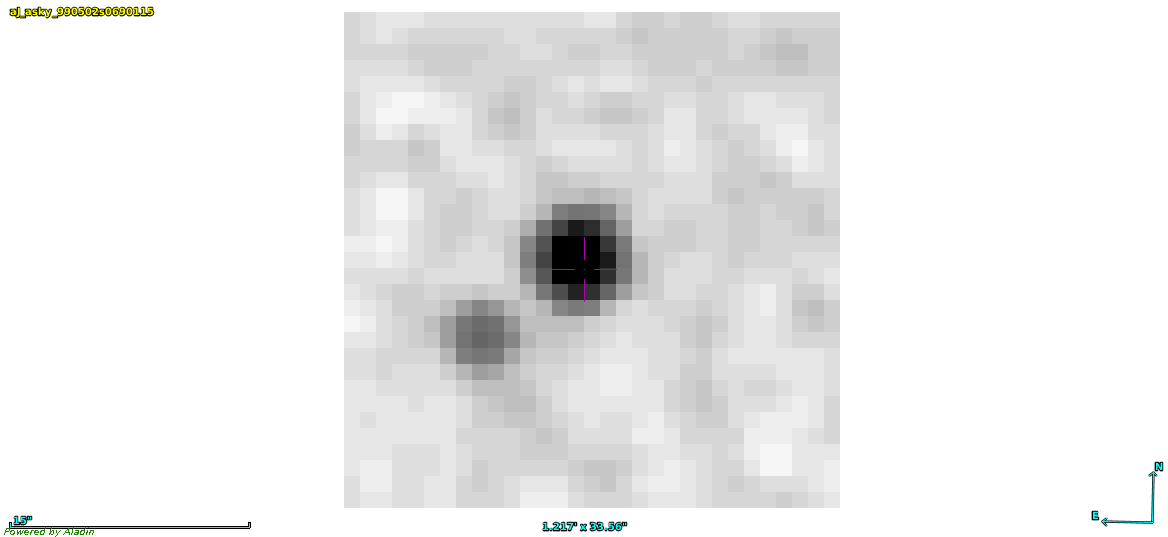
\includegraphics[scale=0.4]{2mass.png}
\caption{\em{image obtained from 2 mass centered on parent dwarf:  RA: 12h07m33.47s dec: -39d32m54.0s  30 arcsec}}
\end{figure}




%-----------------------------Figure Start---------------------------
\begin{figure}[tbh]
% The 'scale' parameter below allows you to scale the figure so that it fits within the page. In this case the figure was scaled to 20% of its original size. Note: for .png files one has to use pdflatex, not classic latex
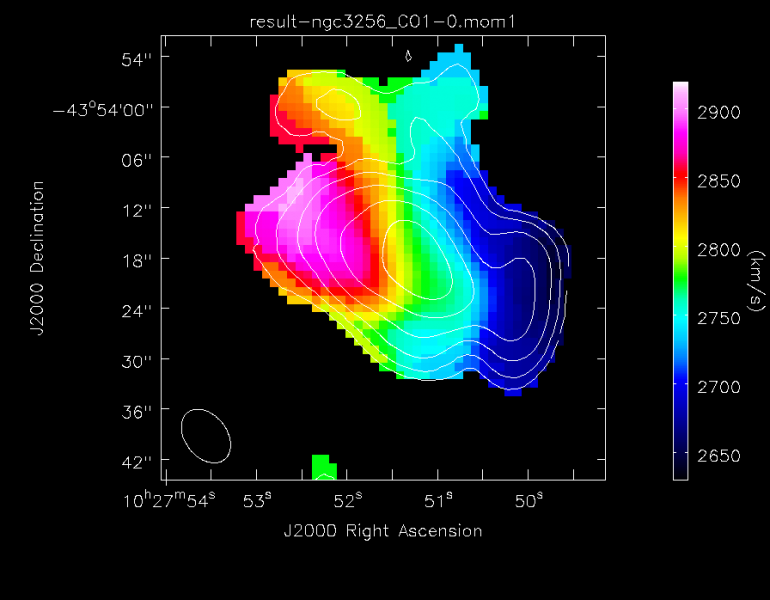
\includegraphics[scale=0.2]{CO_velfield.png}
\caption{\em{The CO(1-0) velocity field of NGC\,3256, with contours 
of the total line emission map overlaid (ALMA Science Verification Data).
}}
\end{figure}
%-----------------------------Figure End------------------------------

%-----------------------------Table Start-----------------------------
\begin{table}[tbh]
\begin{center}
\caption[]{\em{Here we show the continuum sensitivity required per band.}}
\begin{tabular}{cc}
\hline \noalign {\smallskip}
Frequency (GHz) & Sensitivity (mJy) \\
\hline \noalign {\smallskip}
100 & 0.01 \\
300 & 0.10 \\
%\hline \noalign {\smallskip}
\end{tabular}
\end{center}
\end{table}
%-----------------------------Table End ------------------------------

You can structure the scientific justification using the two subsections below (optional).

\subsection{Scientific rationale:}

% Please describe the scientific background of the project,
% pertinent references and previous work relevant to this 
% proposal.

\subsection{Immediate objective:}

% Please describe the observations to be made and their specific
% purpose, with a clear explanation of the need for, and 
% appropriateness of, ALMA Cycle 1 data.  

%%%%%%%%%%%%%%%%%%%%%%%%%%%%%
%% Potential for Publicity %%
%%%%%%%%%%%%%%%%%%%%%%%%%%%%%

\section{Potential for Publicity}

% Here, include a brief statement on the potential of your proposal
% to generate publicity based on the scientific results to be obtained.


%%%%%%%%%%%%%%%%%%%%%%%%
%% References section: %
%%%%%%%%%%%%%%%%%%%%%%%%

\section{References}

% List references here

\noindent [1] Author1 et al. year, journal, vol, page

\noindent [2] Author2 et al. year, journal, vol, page


%%%%%%%%%%%%%%%%%%%%%%%%%%%
%%%%% End of document %%%%%
%%%%%%%%%%%%%%%%%%%%%%%%%%%

\end{document}

